\subsection{Oxford}

Al realizar el experimento, se logró llegar al destino en el ttl 21. De estos, 6 no respondieron. Los ttls que Cimbala reconoció como intercontinentales fueron 6, 10, 13, 14, 20, 21.

\begin{figure}[h!]
  \centering
    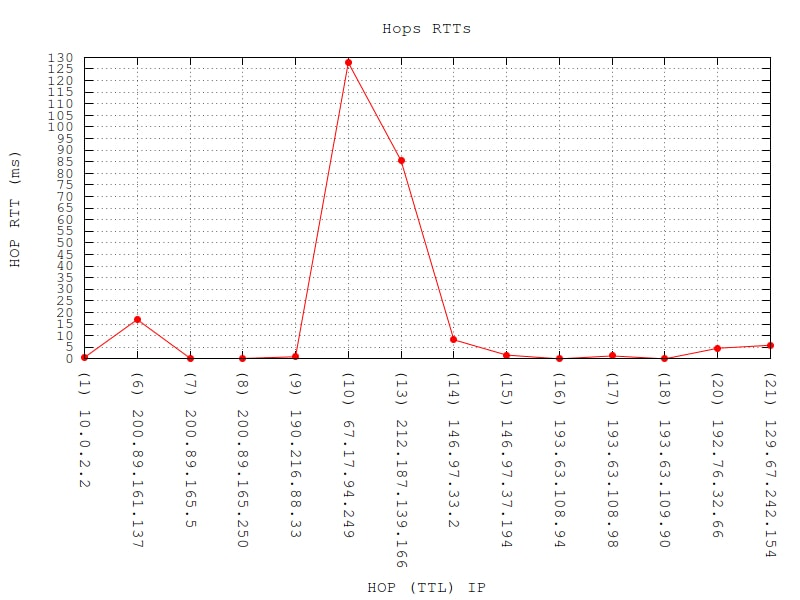
\includegraphics[scale=0.6]{imagenes/oxford-graficos/traceroute-oxford.jpg}
  \caption{Oxford- RTT hops}
  \label{fig:4}
\end{figure}

En la figura \ref{fig:4} se puede observar como el ttl 10, y 13 tienen un rtt claramente distinguido del resto.

\begin{figure}[h!]
  \centering
    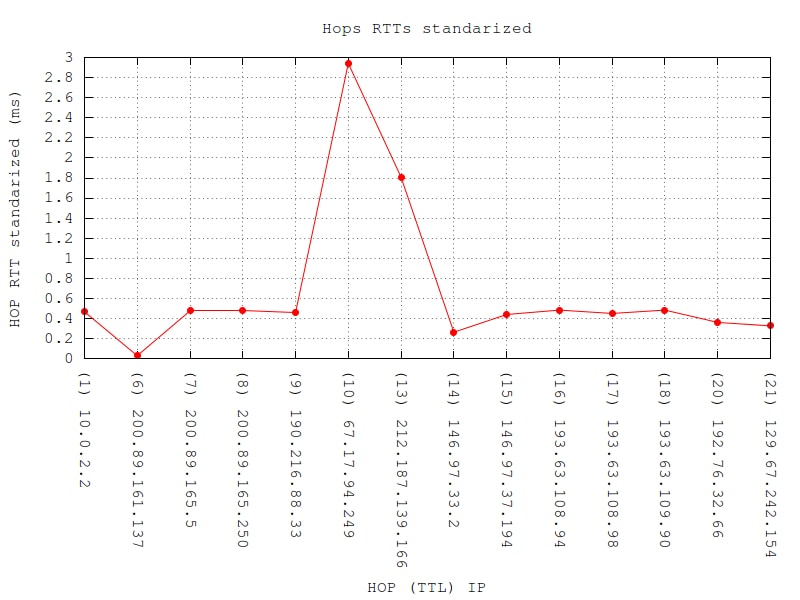
\includegraphics[scale=0.6]{imagenes/oxford-graficos/traceroute-oxford-standarized.jpg}
  \caption{Oxford- RTT hops standarized}
  \label{fig:5}
\end{figure}

En la figura \ref{fig:5} se puede observar una situacion similar a la de la figura \ref{fig:4}.


